
\section{Evaluation}
\label{sec:eval}

Given the prototype constraints discussed in Section~\ref{sec:austere-computing} and my proposed backend architecture, I ask the following question: 
{\em ``Can my flight platform, with severe constraints on both local compute and edge offload, achieve autonomy for active vision?''} Recall, active vision tasks are those that require the drone to react in real time to its surroundings~\cite{Aloimonos1988, Ognibene2013}. To answer this question, I conduct experiments with a series of tasks of increasing difficulty that probe and quantify the limits of my flight platform:

\begin{itemize}

\item{{\bf Task-1:} Detecting a moving object while hovering.}

\item{{\bf Task-2:} Detecting and tracking an object by yawing to keep it in
    the field of view (FOV) as it moves.}

\item{{\bf Task-3:} Detecting and tracking an object by following it at a
    fixed leash distance as the object moves.}

\item{{\bf Task-4:} Detecting a moving object from high altitude, and
    then descending to closely inspect it.  }

\item{{\bf Task-5:} Detecting and avoiding static obstacles.}

\end{itemize}

My goal is to perform these tasks from takeoff to landing with no
human intervention.  Where possible, I test my
system against the Parrot Anafi Ai, a semi-autonomous COTS drone with LTE support, limited onboard tracking and obstacle avoidance.  It weighs more
than twice as much as my flight platform, and costs over five times as much~(Figure~\ref{fig:featurematrix}).  A less-constrained platform
can clearly do more, but it may weigh more too.  My focus is on
whether my 360~g drone-watch platform is too weak or just enough.

The cloudlet used in the following experiments has 36 CPU cores, 128~GB of RAM and an NVIDIA GeForce GTX 1080
Ti GPU.  It is capable of using a private CBRS LTE network for low end-to-end latency. However, since the Galaxy Watch is not able to connect over CBRS, all presented results are based on public cellular network infrastructure.

\subsection{Flight Duration}
\label{sec:flightduration}

Since my platform consists of mounting external components on an
existing drone, a reduction in flight duration is expected. This
reduction is important to quantify, as it directly impacts my
platform's range and practicality. In Figure~\ref{fig:battery}, I
show the hover time of the Parrot Anafi with a 0~g, 40~g, and 60~g
payload weight. The Galaxy Watch with harness is around a 40~g
payload.

\begin{table}
	\centering
	\begin{tabular}{|l|c|c|c|}
		\hline
		& My Platform & Base Parrot Anafi & Parrot Anafi Ai \\
		\hline
		Cost & \$769 & \$469 & \$4,500 \\
		\hline
		Weight & 360~g & 320~g & 898~g \\ 
		\hline
		Detection & \cellcolor{green!30}Yes & \cellcolor{red!30}No & \cellcolor{red!30}No \\
		\hline
		Tracking & \cellcolor{green!30}Yes & \cellcolor{yellow!30}Yes* & \cellcolor{yellow!30}Yes*\\
		\hline
		Avoidance & \cellcolor{green!30}Yes & \cellcolor{red!30}No & \cellcolor{green!30}Yes\\
		\hline
		Programmable & \cellcolor{green!30}Yes & \cellcolor{green!30}Yes & \cellcolor{green!30}Yes\\
		\hline
		4G/5G & \cellcolor{green!30}Yes & \cellcolor{red!30}No & \cellcolor{green!30}Yes\\
		\hline
	\end{tabular}
	\begin{captext}
            \\[0.1cm]
		\centering
		\small *~Requires assistance from the pilot for initial object detection.
	\end{captext}
	\caption{Flight Platforms Relevant to my Experiments}
	\label{fig:featurematrix}
\end{table}

\begin{table}
\centering
\begin{tabular}{|l|c|c|c|c|c|c|}
\hline
&0~g &40~g &\cellcolor[HTML]{FF9470}\% Reduction 
 &60~g &\cellcolor[HTML]{FF9470}\% Reduction \\
 \hline
Battery 1 & 21:04 & 18:43 &11.16\% & 17:18 &17.88\% \\
 \hline
Battery 2 & 22:54 & 19:35 &14.48\% & 18:57 &17.25\% \\
 \hline
Battery 3 & 17:57 & 14:23 &19.87\% & 13:00 &27.58\% \\
 \hline
Battery 4 & 20:00 & 16:43 &16.42\% & 15:12 &24.00\% \\
 \hline
\end{tabular}
\caption{Flight Duration by Payload Weight}
\label{fig:battery}
\end{table}

\subsection{Event-to-Detection Latency}
\label{sec:event-to-detection-latency}

The agility of my system is limited by the end-to-end latency of the
processing pipeline~(Figure~\ref{fig:sys-arch}).  Events closer in
time than this limit may not be resolvable.  For example, a
surveillance target with a jerky motion will be perceived as moving
more smoothly.  Large, but brief, deviations from the smoothed path
may not be detected.  The larger the end-to-end latency, the greater
the need for predictive approaches in tracking fast-moving
targets.  This, in turn, leads to greater likelihood of errors due
to mis-prediction.

The base end-to-end latency of the pipeline can by replicating the experiment described in Section~\ref{sec:streaming-experiment-setup} and Figure~\ref{fig:streaming-experiment}. The
drone is kept stationary in a lab setting, with its camera pointing at a display attached to the cloudlet. Except
for the fact that the drone is not flying, everything else (hardware, software, and network) is identical to Figure~\ref{fig:sys-arch}.  The cloudlet-connected display shows the current time at millisecond
granularity.  An image of this timestamp is captured by the drone's camera, transmitted downstream, and recovered at the end of the pipeline.  Its difference from current time at recovery gives the end-to-end latency.  Figure~\ref{fig:e2elatency} presents my results from 30 samples. The distribution is heavy-tailed, with a mean of 1138~ms and a standard deviation of 157~ms.  The high mean and variability arise from jitter in LTE transmission, as well as from processing and scheduling delays on the drone, watch, and cloudlet.


\begin{figure}
\centering
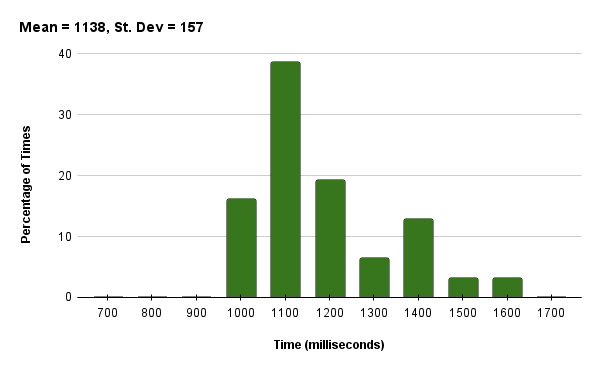
\includegraphics[width=0.7\linewidth]{chapter4/FIGS/new_mtp_watch.png}
\caption{Distribution of Detection Latency (Galaxy Watch)}
\label{fig:e2elatency}
\end{figure}


\subsection{Task-1: Object Detection While Hovering}
\label{sec:task1}

\subsubsection{Task Description}
\label{sec:task1-desc}

The accuracy of the computer vision pipeline complements its speed.
\begingroup
\setlength{\columnsep}{4pt}
Both are important for active vision.  A simple test is the detection
of a target on the ground when it moves into the camera's FOV.  The
problem is harder from higher altitude because objects are smaller and
DNNs perform poorly on objects that are just a few pixels in
size~\cite{Huang2017}.
Figure~\ref{fig:robomaster} shows the DJI Robomaster S1
robot~\cite{Robomaster2022} used as the detection target in my
experiments.  It is roughly the size of a small dog, and can be
remote-controlled over WiFi by a human driver.  It can also be
programmed to follow a predefined route, with speed variation in
different route segments. 

\begin{figure}
\centering
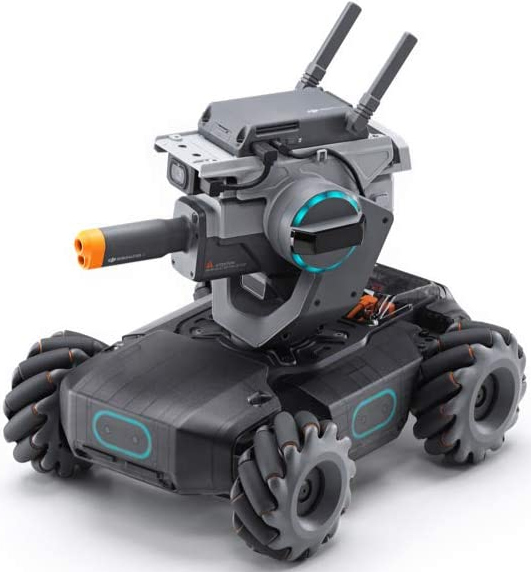
\includegraphics[width=0.2\linewidth]{chapter4/FIGS/robomaster.jpg}\\
{\footnotesize 432~x~330~x~304~mm\\[-0.05in]
\noindent(17~x~13~x~12~in)}
\caption{COTS Target}
\label{fig:robomaster}
\end{figure}

For Task-1, the robot is manually operated
on a freeform path that overlaps the FOV of the drone that is hovering
at fixed altitude.  In postprocessing, I compare ground truth~(GT) on
each processed frame with the output of the processing pipeline.  The
object detection DNN was created via transfer learning from
SSD-ResNet50~\cite{SSDResnet50} pre-trained on the COCO dataset.  The
training set was created from drone-captured images of the target
shown in Figure~\ref{fig:robomaster}.

\endgroup


\subsubsection{Results}
\label{sec:task1-results}

I perform this experiment at altitudes of 5~m, 10~m, and 15~m.
Accuracy is high at 5~m; a typical result is
Figure~\ref{fig:task1-images}(a), where the bounding box indicates
detection followed by correct target classification at high
confidence~(0.98).  The person at the top right and the distractor
object at the top middle are correctly ignored.  At 10~m, accuracy is
slightly lower.  An example of an erroneous result at 10~m is
Figure~\ref{fig:task1-images}(b), which shows a true positive~(TP)
(the target) at confidence 0.95 at bottom center, and a false
positive~(FP) (a person misclassified as the target at confidence
0.82) at center left.  At 15~m, accuracy suffers significantly.  An
example of an error at 15~m is Figure~\ref{fig:task1-images}(c).  This
shows an FP at center right (a person misclassified as the
target at confidence 0.86), and also a false negative~(FN) (missed target)
at center left.  Altitudes of 15~m and higher are clearly challenging
for this combination of target size, optical system, and processing pipeline.

\begin{figure}
\centering\small
\centering
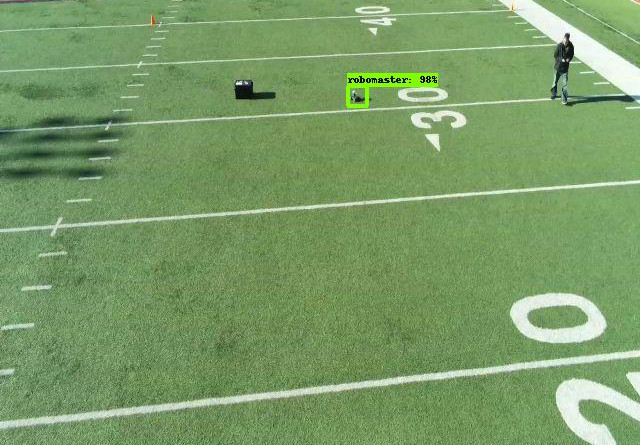
\includegraphics[width=0.6\linewidth]{chapter4/FIGS/fig-static-detection-example2-5m.jpg}\\
(a) Altitude = 5m\\[0.1in]
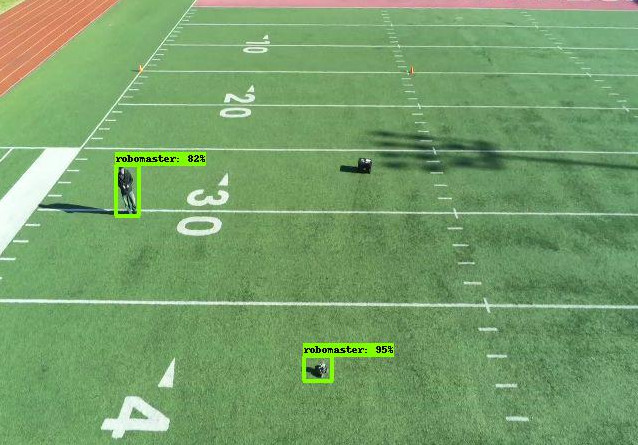
\includegraphics[width=0.6\linewidth]{chapter4/FIGS/fig-static-detection-example2-10m.jpg}\\
(b) Altitude = 10m\\[0.1in]
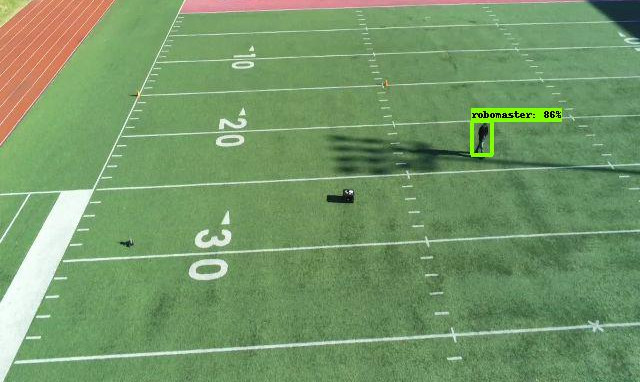
\includegraphics[width=0.6\linewidth]{chapter4/FIGS/fig-static-detection-example2-15m.jpg}\\
(c) Altitude = 15m
\caption{Task-1 Images}
\label{fig:task1-images}
\end{figure}

Table~\ref{tab:task1-results}~(a) shows the confusion matrix for
Task-1 at a confidence threshold of 0.7.  The scoring of images used
in this matrix requires explanation. Classic measures of precision and
recall address scene classification, where an entire image is
correctly or incorrectly classified.  In contrast, my setting
involves object detection.  It is possible for a single image to have
both a FP and a TP or FN.  Figure~\ref{fig:task1-images}(a) contains
a single TP, and no errors.  This is scored as a TP in the confusion
matrix.  Figure~\ref{fig:task1-images}(b) contains both a TP and an
FP; this is scored as an FP since errors trump correctness.  When
there are multiple errors, the worst error determines the score.
Figure~\ref{fig:task1-images}(c), for example, contains both an FP and
an FN.  I view FNs (hurting recall) as more serious errors than FPs
(hurting precision), and therefore score the whole image as an FN.
These rules preserve the invariant
$$GT_P + GT_N = TP + TN + FP + FN$$
where $GT_P$ and $GT_N$ refer to ground truth positives and negatives,
and TN refers to true negatives (no target in image).

\begin{table}
\centering\small
\begin{minipage}[b]{2.4in}
\centering\small
\begin{tabular}{|c|c|c|c|c|}
\hline
Alti-&\multicolumn{2}{c|}{Ground}&\multicolumn{2}{c|}{Detected}\\
\cline{4-5}
tude&\multicolumn{2}{c|}{Truth}& Pos& Neg.\\
\hline
5 m & Pos. & 85 & 71 & 13\\
    & Neg. &  0 & 1  & 0\\
\hline
10 m & Pos. & 90 & 55 & 30\\
     & Neg. &  0 & 5  & 0 \\
\hline
15 m & Pos. & 85 & 24 & 48 \\
     & Neg. &  0 & 13 & 0\\
\hline
\end{tabular}\\[0.05in]
{\footnotesize Threshold = 0.7}\\
(a) Confusion Matrix\\
\end{minipage}
\begin{minipage}[b]{1.4in}
\centering
\begin{tabular}{|c|c|c|}
\hline
Alti-& Prec- & Re-\\
tude & ision & call\\
\hline
5 m & 0.99 & 0.85 \\
10 m &0.92 & 0.65\\
15 m & 0.65 & 0.33 \\
\hline
\end{tabular}\\[0.05in]
(b) Precision and Recall
\end{minipage}

\caption{Task-1 Results}
\label{tab:task1-results}
\vspace{-0.2in}
\end{table}


At 5~m, a total of 85 frames are processed.  The column labeled
``Ground Truth'' shows that all 85 contain a target instance.  The
``Detected'' columns show that 71 out of the 85 are correctly detected
and classified~(TPs), but 13 are missed~(FNs).  At 10~m, all 90
processed frames contain an instance of the target, but only 55 of
them are correctly detected~(TPs).  There are 30~FNs and 5~FPs.  At
15~m, accuracy suffers considerably.  Out of 85 total processed
frames, all are GT-positive.  However, only 24 of them are correctly
detected~(TPs).  There are 48~FNs and 13~FPs.
Table~\ref{tab:task1-results}~(b) shows the precision and recall
resulting from this confusion matrix.  These values are excellent at
5~m.  Recall is noticeably degraded at 10~m.  Both precision and
recall suffer at 15~m.  These results suggest the importance of active
vision. Dropping to a lower altitude could confirm
or refute the sighting of an object from higher altitude. 

\subsection{Task-2: Keeping Sight of  a Moving Object}
\label{sec:task2}

\subsubsection{Task Description}
\label{sec:task2-desc}

Processing a frame in Task-1 does not lead to actuation of the drone.
In contrast, Task-2 represents a simple form of active vision. After
detecting a moving target, the drone yaws to keep the target visible
in the frame. There is no forward or backward motion, only rotation to
keep the object in the FOV. To find the target in frame,  Target speed and motion predictability
clearly influence this task.  A fast-moving target that unpredictably
and frequently changes its path is clearly hard to track.  As
discussed earlier~(\S~\ref{sec:event-to-detection-latency}), the end-to-end latency of
processing constrains tracking agility. With the help of the pilot
(using the FreeFlight app), the Anafi Ai can also perform this task
and thus I use it as a benchmark for my platform.

\begingroup
\setlength{\columnsep}{4pt}
\begin{figure}
\centering
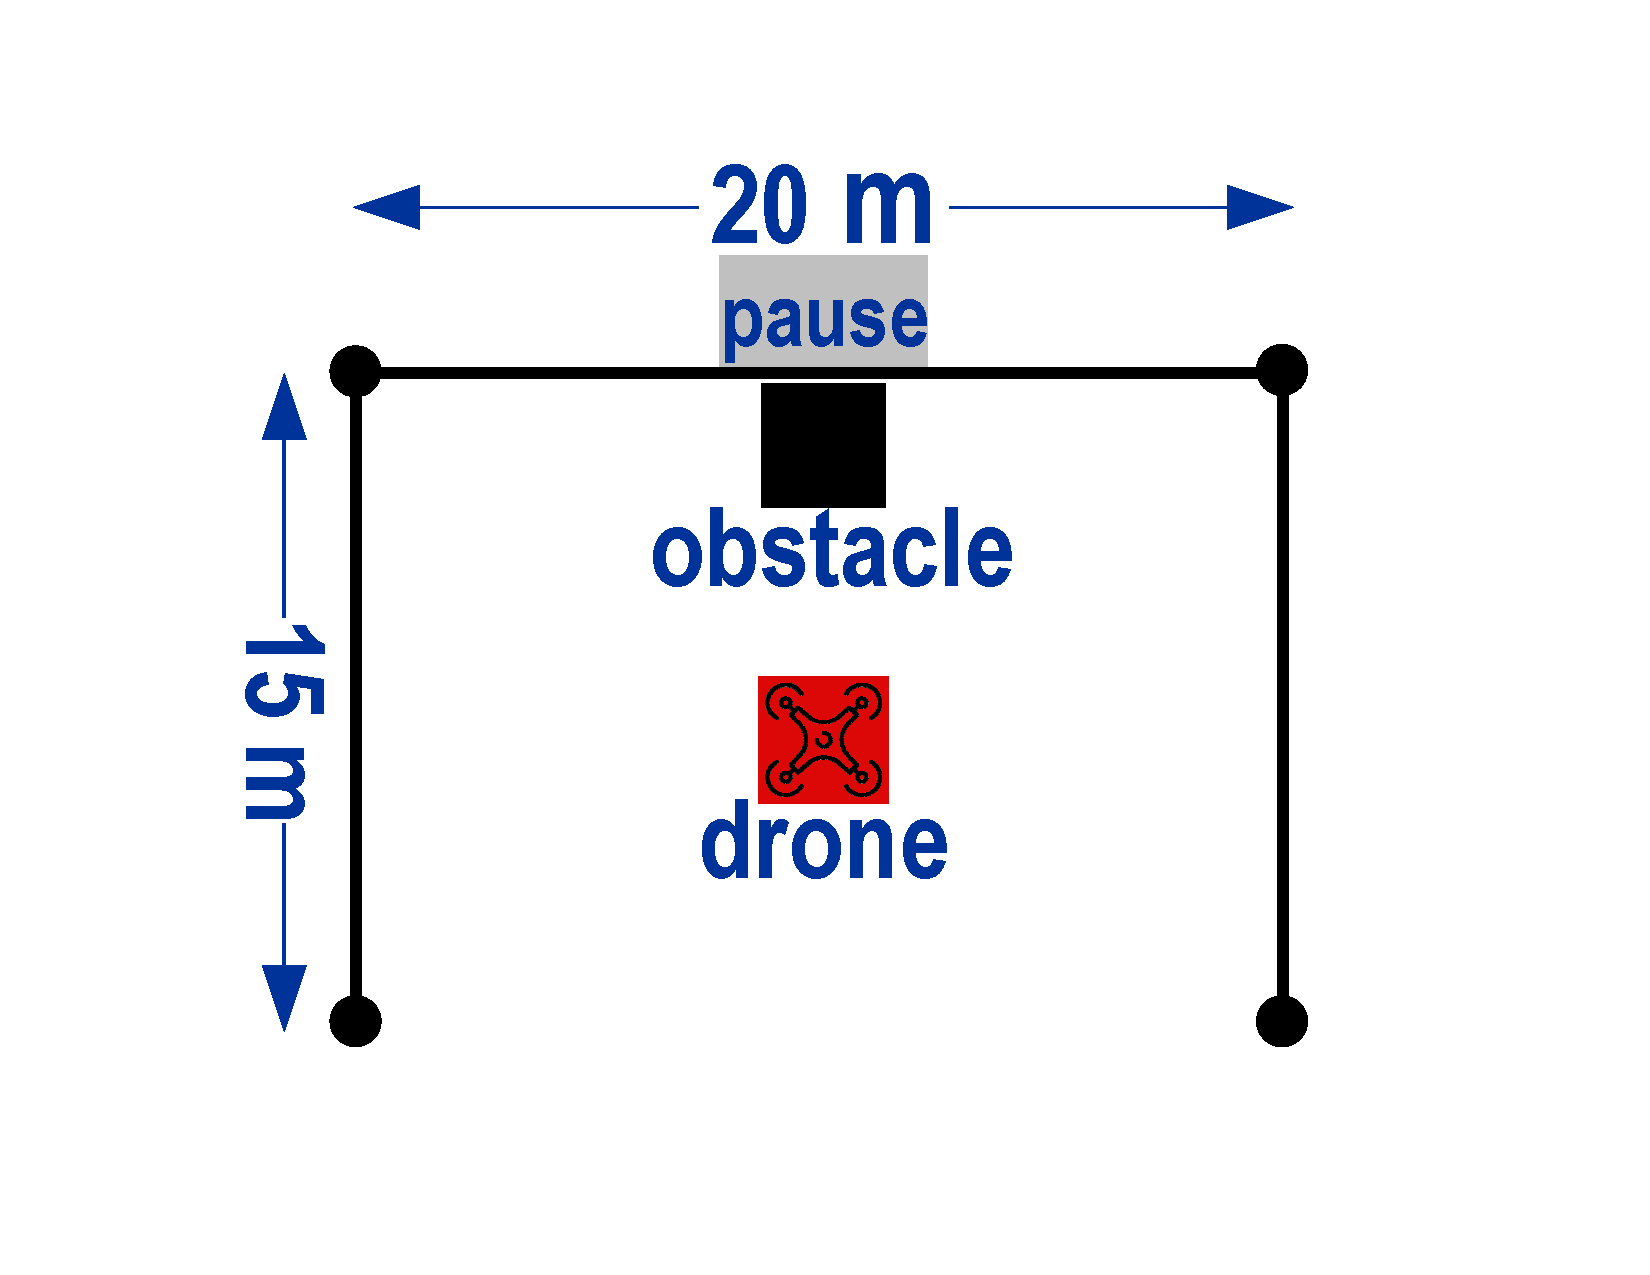
\includegraphics[width=0.4\linewidth]{chapter4/FIGS/fig-yaw-ushape.pdf}\\
\caption{Target Occlusion}
\label{fig:yaw}
\end{figure}

As shown in Figure~\ref{fig:yaw}, I set up a rectangular
(approximately 20~m~x~15~m) course marked by 4 cones.  The drone is
placed near the center of the rectangle and takes off to a fixed
altitude of 2 meters. A 2~m tall by 0.5~m wide foam pillar is placed
to occlude the target along the center of the back edge. For each run,
the target moves along the right, back, and left edges in a u-shape
two times. To test the ability of each platform to reacquire lost
targets, I vary the time spent being occluded, starting with no
pause, then pausing for 2 seconds behind the pillar, and finally a 5
second pause. Three runs of each delay were recorded.  For the Anafi
Ai, the pilot must draw a bounding box around the target in order to
start tracking; my platform automatically acquires and re-acquires
the target.  Since my platform is constrained to below 1~fps, we
compare results from the two platforms on frames that are one second
apart.  The Anafi Ai captures video at 30~fps, so I expect its
responsiveness in this task to be significantly better.

\subsubsection{Algorithm}
\label{sec:tracking-algorithm-basic}
Edge offload to a powerful cloudlet enables tracking via DNN
inferencing on every frame received.  This ``brute force'' approach
eliminates the need for predictive heuristics, such as those based on
optical flow algorithms.  Heuristics are often needed by on-board
tracking implementations because the computational demand would
otherwise be too high.  The brute force approach makes tracking robust
with respect to transient occlusions.  Flow-based approaches, in
contrast, are typically unable to reacquire the target after occlusion
ends.

In my system, the cloudlet inferences each frame through an object
detection DNN. The highest confidence bounding box is then chosen as
the target, and its offset from the center of the frame is calculated
in field-of-view degrees. The drone then actuates according to a
PID-loop~\cite{Ang2005} based on the offset error.  This simple
approach provides a good baseline at low complexity.

\begin{table}
	\centering\small
	\begin{tabular}{|c|c|c|c|c|c|c|}
		\hline
		 &  &  & \multicolumn{2}{c|}{Success} & Slow & \\
		Delay & Run & Total  & \multicolumn{2}{c|}{\footnotesize (Target Present)} & Act- &  Fail\\
		\cline{5-5} 
		(s)&  &       Frames  &         & $\rm \frac{Present}{Total}$ & uation  & \\ 
		\hline
		& 1 & 63 & 60 & & 3 & 0 \\
		0 & 2 & 62 & 62 & 91.2\% \scriptsize{(11.4\%)}  & 0 & 0 \\
		& 3 & 60 & 47 & & 0 & 13\\
		\hline
		& 1 & 58 & 56 & & 2 & 0 \\
		2 & 2 & 58 & 57 & 98.3\% \scriptsize{(1.7\%)} & 1 & 0 \\
		& 3 & 64 & 64 & & 0 & 0 \\
		\hline
		& 1 & 59 & 53 & & 0 & 6 \\
		5 & 2 & 53 & 53 & 90.3\% \scriptsize{(9.4\%)} & 0 & 0  \\
		& 3 & 53 & 43 & & 0 & 10 \\
		\hline
	\end{tabular}
	\begin{captext}
		\centering \\[0.1cm] \small Figures in parentheses are standard deviations. \\
	\end{captext}
{(a) My Platform}\\[0.2in]

\begin{tabular}{|c|c|c|c|c|c|c|}
\hline
		 &  &  & \multicolumn{2}{c|}{Success} & Slow & \\
Delay & Run & Total  & \multicolumn{2}{c|}{\footnotesize (Target Present)} & Act- &  Fail\\
\cline{5-5} 
(s)&  &       Frames  &         & $\rm \frac{Present}{Total}$ & uation  & \\ 
\hline
    & 1 & 76 & 76 &    & 0 & 0 \\
0 & 2 & 78 & 78 & 100\% \scriptsize{(0\%)} & 0 & 0 \\
    & 3 & 80 & 80 &    & 0 & 0 \\
\hline
    & 1 & 79 & 79 &        & 0 & 0 \\
2 & 2 & 80 & 80 & 100\% \scriptsize{(0\%)} & 0 &  0 \\
    & 3 & 86 & 86 &        & 0 &  0 \\
\hline
    & 1 & 78 & 32 &        & 0 &  46 \\
5 & 2 & 77 & 29 & 39.4\% \scriptsize{(1.7\%)} & 0 & 48 \\
    & 3 & 81 & 32 &        & 0 &  49 \\
\hline
\end{tabular}
\begin{captext}
\centering \\[0.1cm] \small Figures in parentheses are standard deviations. \\
\end{captext}
{(b) Anafi Ai}

\caption{Task-2 Results}
\label{tab:task2-results}
\end{table}

\subsubsection{Results}
\label{sec:task2-results}
For successful tracking, both sensing and actuation are important.  If
the drone is sluggish in executing a yaw command, even perfect
processing may not keep the target in the FOV at all times.
Four outcomes are possible for each processed frame:
\begin{itemize}
	\item{the target is visible in the frame ({\small ``Success''}).}
	
	\item{the target is missing in this frame because of slow actuation, but present in the next ({\small ``Slow Actuation''}).}
	
	\item{the target is missing both in this frame and the next.
		This is scored as a tracking failure ({\small ``Fail''}).}
	
	\item{the target is occluded.
		This is not included in the frame total and is omitted from the results.}
\end{itemize}


Table~\ref{tab:task2-results}(a) and (b) compare the results for my
platform and the Anafi Ai.  At 0~s occlusion, my platform performs
well, but run 3 experiences some tracking failures.  My system's low
framerate stream accounts for these failures.  None of the frames
received by the cloudlet included the target as it traversed the last
corner of the pattern.  In contrast, the Anafi Ai experiences no
failures at 0~s occlusion.  At 2~s occlusion, both my platform and
the Anafi Ai perform very well.  However, my platform experiences a
few instances of slow actuation.  Both platforms are able to reliably
reacquire the target as it reappears from behind the obstacle.  At 5~s
occlusion, the limitations of the Anafi Ai are exposed. Such a long
period of occlusion causes the Ai's optical flow tracking algorithm to
become confused, often mistaking the pillar or background objects for
the target. my platform's DNN tracking handles the increased
occlusion well, with only a modest increase in the number of failures.

\begin{figure}
\begin{minipage}{0.5\linewidth}
\centering
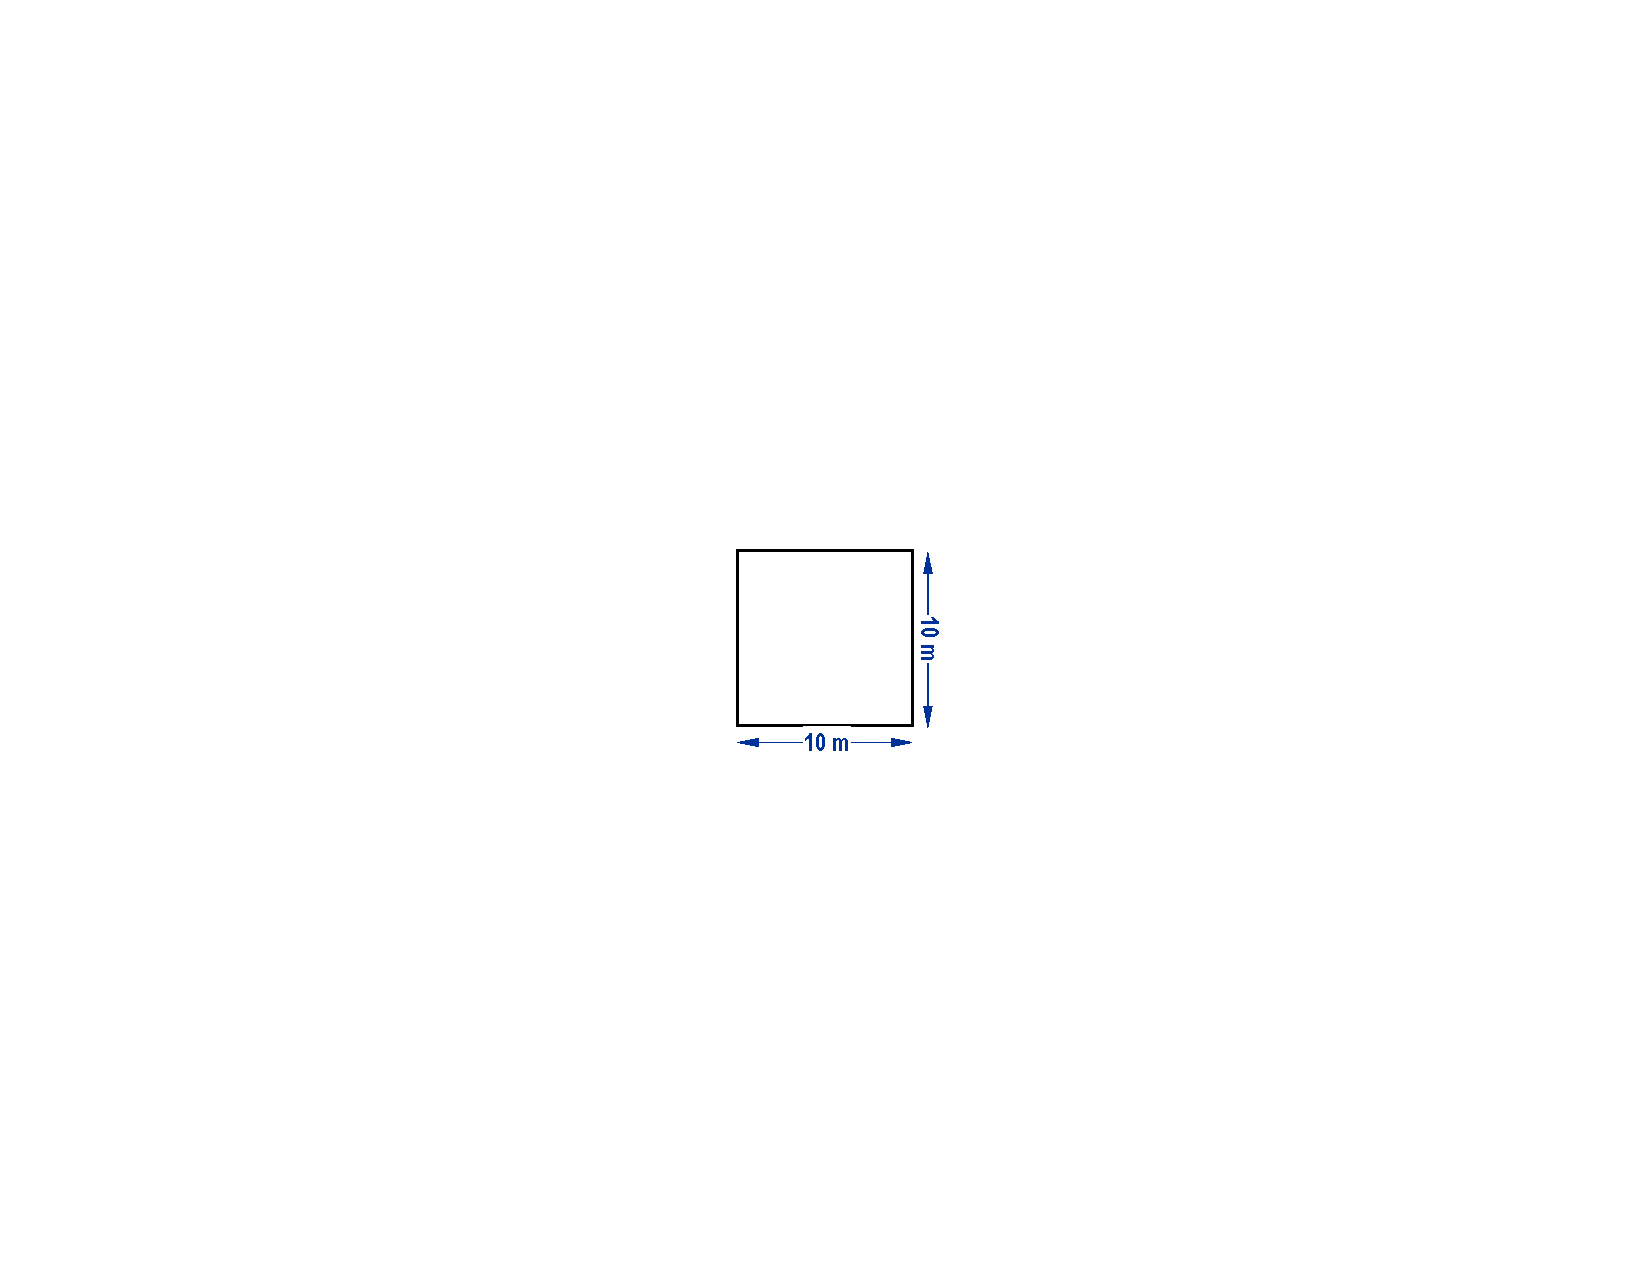
\includegraphics[width=0.6\linewidth]{chapter4/FIGS/fig-pattern-square.pdf}\\
{(a) Square}\\
\end{minipage}
\begin{minipage}{0.5\linewidth}
\centering
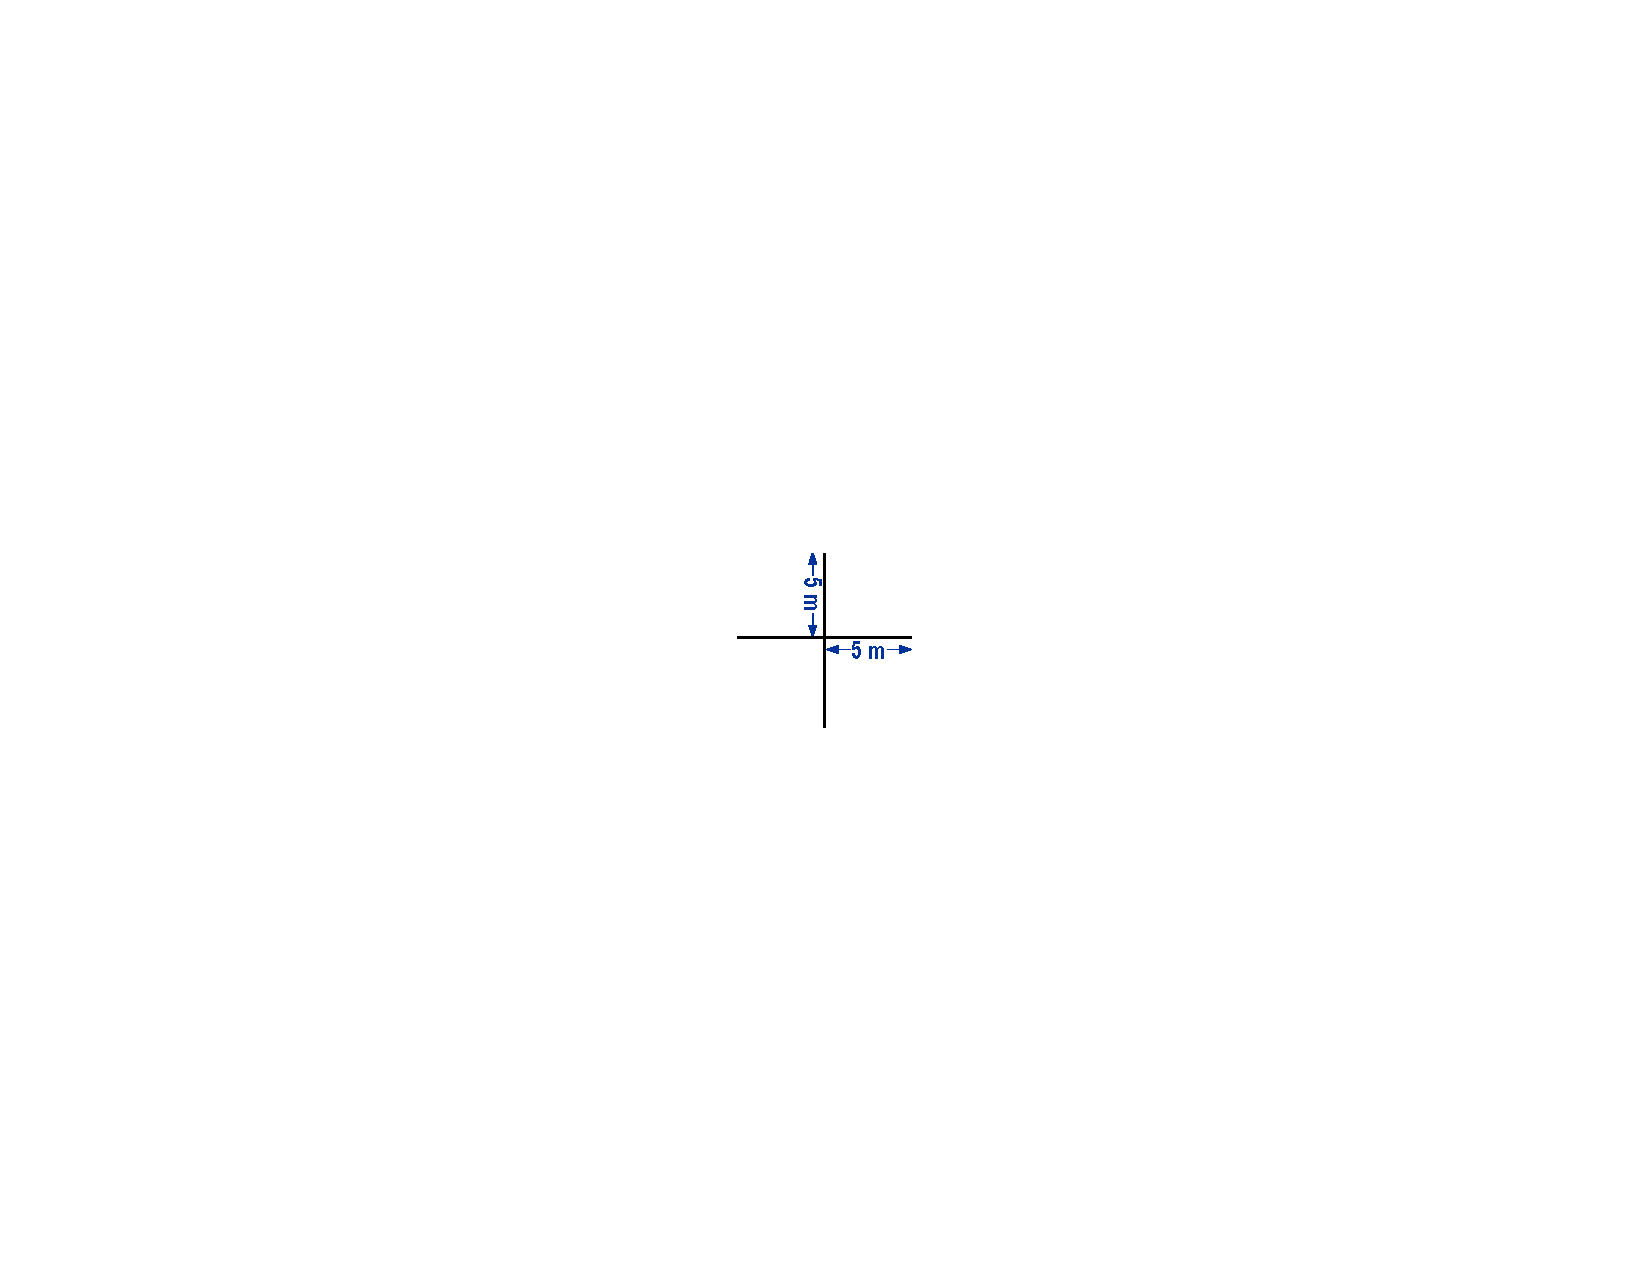
\includegraphics[width=0.6\linewidth]{chapter4/FIGS/fig-pattern-cross.pdf}\\
{(b) Cross}\\
\end{minipage}
\caption{Tracking Patterns}
\label{fig:patterns}
\end{figure}

\subsection{Task-3: Following at a Fixed Leash Distance}
\label{sec:task3}

\subsubsection{Task Description}
\label{sec:task3-desc}

Only limited actuation is needed to keep the target in the
drone's FOV in Task-2.  More substantial actuation is required for
Task-3.  After detecting a moving target, the drone moves to keep it
at a preset {\em leash distance.} This compounds latency issues as the
drone must now yaw and reposition itself correctly when the target
maneuvers quickly. At high target speeds (over 2.5~m/s), this can
prove difficult because even small actuation mistakes can result in
total loss of visual contact. Although the Anafi Ai can statically
track moving objects, it does not have a 
following feature which makes a direct comparison of its performance infeasible.

I programmed the target to move at a constant speed over flat ground
in a specified pattern.  I used speeds of 1.5~m/s (slow), 2.5~m/s
(medium), and 3.5~m/s (fast).  These speeds roughly correspond to a
person walking, jogging slowly, and running.  Two patterns were used:
a square of side 10~m~(Figure~\ref{fig:patterns}(a)), and a cross with
four arms of 5~m each~(Figure~\ref{fig:patterns}(b)).  The square
embodies abrupt change of trajectory after 10~m of straight line travel,
while the change of trajectory in the cross occurs after only 5~m. As in Task-1, the drone is initially hovering at fixed altitude.  I used altitudes of 5~m and 10~m in my experiments, but omitted 15~m
since Section~\ref{sec:task1-results} indicates poor performance at this altitude. 

\subsubsection{Algorithm}
\label{sec:tracking-algorithm-advanced}
The algorithm used for this experiment is a modified version of the one used in Section~\ref{sec:task2}. Once the target is detected, the drone tracks it by centering the bounding box in the frame. At the same time, it estimates its distance to the target, and moves such that it preserves a preset \textit{leash distance}. This leash distance is chosen before the experiment to adequately frame the target at the specified altitude. If the drone loses sight of the target, it hovers until
the object moves back into its FOV. No active search is made
by the drone to reacquire a lost target.

\subsubsection{Results}
\label{sec:task3-results}

I use the same scoring rubric of ``Success,'' ``Slow Actuation,'' and
``Fail'' as for Task-2.  At a target speed of 1.5~m/s, the results for
all runs in Table~\ref{tab:task3-results-5m-square} confirm
successful tracking with only occasional failure.  When speed
increases to 2.5~m/s, and then to 3.5~m/s, the number of failures
increases sharply.  This is consistent with the computer vision
processing pipeline following real-world scene changes too slowly, due
to the very low frame rate~(0.7~fps).  I show
later~(\S\ref{sec:discussion-results}) that increasing frame rate
improves tracking.  The effects of anomalously high LTE latency are
visible in Run 3.  This points to the challenge of using public
cellular networks which can experience unpredictable changes in bandwidth and latency.

\begin{table}
	\centering\small
	\begin{tabular}{|c|c|c|c|c|c|c|}
		\hline
		Speed & Run & Total & \multicolumn{2}{c|}{Success} & Slow & Fail\\
		(m/s) &  & Frames  & \multicolumn{2}{c|}{\footnotesize (Target Present)} & Act- &  \\
		\cline{5-5} 
		&  &         &         & $\rm \frac{Present}{Total}$ & uation  & \\ 
		\hline
		& 1 & 82 & 80 & & 1 & 1 \\
		1.5 & 2 & 85 & 76 & 95.2\% \scriptsize{(5\%)}  & 0 & 9 \\
		& 3 & 77 & 76 & & 1 & 0\\
		\hline
		& 1 & 82 & 49 & & 2 & 31 \\
		2.5 & 2 & 84 & 50 & 55\% \scriptsize{(8\%)} & 4 & 30 \\
		& \cellcolor{red!30}3 & \cellcolor{red!30}83 & \cellcolor{red!30}38 & & \cellcolor{red!30}0 & \cellcolor{red!30}45 \\
		\hline
		& 1 & 87 & 46 & & 2 & 39 \\
		3.5 & 2 & 84 & 60 & 62.7\% \scriptsize{(9.3\%)} & 1 & 23  \\
		& 3 & 83 & 53 & & 4 & 26 \\
		\hline
	\end{tabular}
	\begin{captext}
		\centering \\[0.1cm] Figures in parentheses are standard deviations.\\
		Abnormally high LTE latency was observed during the red highlighted run. This is always a possibility when using public cellular infrastructure. During high latency events, the performance of the system suffers considerably.
	\end{captext}
	\caption{Task-3 Results {\small (Altitude = 5~m, Pattern = Square)}}
	\label{tab:task3-results-5m-square}
\end{table}


Table~\ref{tab:task3-results-5m-cross} presents Task-3 results when
the pattern used is a cross rather than a square.  Comparing the
``Fail'' columns of Tables~~\ref{tab:task3-results-5m-square} and
\ref{tab:task3-results-5m-cross}, there is a noticeable decrease in
failures at speeds of 2.5~m/s and 3.5~m/s when the pattern is a cross.
These results are consistent with the cross being less demanding than
the square for tracking.

\begin{table}
\centering\small
\begin{tabular}{|c|c|c|c|c|c|c|}
\hline
Speed & Run & Total & \multicolumn{2}{c|}{Success} & Slow & Fail\\
(m/s) &  & Frames  & \multicolumn{2}{c|}{\footnotesize (Target Present)}& Act-  &  \\
\cline{5-5} 
      &  &         &         & $\rm \frac{Present}{Total}$ & uation  & \\ 
\hline
    & 1 & 83 & 83 &    & 0 & 0 \\
1.5 & 2 & 88 & 88 & 100\% \scriptsize{(0\%)} & 0 & 0 \\
    & 3 & 78 & 78 &    & 0 & 0 \\
\hline
    & 1 & 85 & 67 &        & 0 & 18 \\
2.5 & 2 & 80 & 75 & 88.6\% \scriptsize{(8.5\%)} & 0 &  5 \\
    & 3 & 88 & 82 &        & 1 &  5 \\
\hline
    & 1 & 82 & 82 &        & 0 &  0 \\
3.5 & 2 & 85 & 59 & 89\% \scriptsize{(17\%)} & 1 & 25 \\
    & 3 & 86 & 84 &        & 2 &  0 \\
\hline
\end{tabular}
\begin{captext}
\centering \\[0.1cm] Figures in parentheses are standard deviations. \\
\end{captext}
\caption{Task-3 Results {\footnotesize (Altitude = 5~m, Pattern = Cross)}}
\label{tab:task3-results-5m-cross}
\end{table}

\begin{table}
	\centering\small
	\begin{tabular}{|c|c|c|c|c|c|c|}
		\hline
		Speed & Run & Total & \multicolumn{2}{c|}{Success} & Slow & Fail\\
		(m/s) &  & Frames  & \multicolumn{2}{c|}{\footnotesize (Target Present)}& Act-  &  \\
		\cline{5-5} 
		&  &         &         & $\rm \frac{Present}{Total}$ & uation  & \\ 
		\hline
		& 1 & 83 & 65 & & 1 & 17 \\
		1.5 & 2 & 78 & 74 & 81.6\% \scriptsize{(12\%)}  & 0 & 4 \\
		& 3 & 88 & 63 & & 3 & 19\\
		\hline
		& 1 & 82 & 52 & & 2 & 39 \\
		2.5 & 2 & 83 & 48 & 62.3\% \scriptsize{(4\%)} & 1 & 34 \\
		& 3 & 87 & 57 & & 0 & 30 \\
		\hline
		& 1 & 88 & 57 & & 1 & 30 \\
		3.5 & 2 & 83 & 45 & 64.8\% \scriptsize{(10.5\%)} & 1 & 37  \\
		& 3 & 89 & 67 & & 3 & 19 \\
		\hline
	\end{tabular}
	\begin{captext}
		\centering \\[0.1cm] Figures in parentheses are standard deviations. \\
	\end{captext}
	\caption{Task-3 Results {\footnotesize (Altitude = 10~m, Pattern = Square)}}
	\label{tab:task3-results-10m-square}
\end{table}


At an altitude of 10~m, the drone's FOV is increased, but there is a
significant drop in precision and recall as shown in
Table~\ref{tab:task1-results}~(b).  This leads to an increase in the
number of tracking failures relative to 5~m, regardless of the target
pattern or speed.  The effect is most apparent at the slowest speed:
the results for 1.5~m/s in Table~\ref{tab:task3-results-10m-square}
show higher failures than the results at 1.5~m/s in
Table~\ref{tab:task3-results-5m-square}.  Similarly, the results for
1.5~m/s in Table~\ref{tab:task3-results-10m-cross} show higher
failures than the results for 1.5~m/s in
Table~\ref{tab:task3-results-5m-cross}. These effects persist at
higher speeds, but are less obvious.  The improvement at
2.5~m/s between Tables~\ref{tab:task3-results-5m-square} and
\ref{tab:task3-results-10m-square} is due to the high-latency LTE
anomaly mentioned earlier.

\begin{table}
	\centering\small
	\begin{tabular}{|c|c|c|c|c|c|c|}
		\hline
		Speed & Run & Total & \multicolumn{2}{c|}{Success} & Slow & Fail\\
		(m/s) &  & Frames  & \multicolumn{2}{c|}{\footnotesize (Target Present)}& Act-  &  \\
		\cline{5-5} 
		&  &         &         & $\rm \frac{Present}{Total}$ & uation  & \\ 
		\hline
		& 1 & 80 & 75 &    & 0 & 5 \\
		1.5 & 2 & 85 & 85 & 87.3\% \scriptsize{(16.8\%)} & 0 & 0 \\
		& 3 & 85 & 58 &    & 0 & 27 \\
		\hline
		& 1 & 84 & 67 &        & 0 & 17 \\
		2.5 & 2 & 81 & 81 & 86.6\% \scriptsize{(11.6\%)} & 0 &  0 \\
		& 3 & 85 & 68 &        & 0 &  17 \\
		\hline
		& 1 & 86 & 62 &        & 0 &  24 \\
		3.5 & 2 & 86 & 85 & 82.9\% \scriptsize{(14.1\%)} & 1 & 0 \\
		& 3 & 86 & 67 &        & 1 &  18 \\
		\hline
	\end{tabular}
	\begin{captext}
		\centering \\[0.1cm] Figures in parentheses are standard deviations. \\
	\end{captext}
	\caption{Task-3 Results {\footnotesize (Altitude = 10~m, Pattern = Cross)}}
	\label{tab:task3-results-10m-cross}
\end{table}

\subsection{Task-4: Close Inspection}
\label{sec:task4}

\subsubsection{Task Description}
\label{sec:task4-desc}

Task-4 corresponds to the classic active vision tactic of ``taking a
closer look'' that was mentioned earlier~(\S\ref{sec:introduction}).   It
begins with the drone hovering at 15~m.  As in Task-1, the target
moves in a freeform path that is manually controlled over WiFi.  When
the target is detected in the FOV of the drone, confirmation at the
lower altitude of 5~m is attempted.  During the descent, the target is
kept in the FOV using yaw and gimbal actuation; the drone's
pitch and roll are not modified.  If multiple targets are detected at
15~m, only confirmation of the highest-confidence detection is
attempted.



\subsubsection{Results}
\label{sec:task4-results}

The results for Task-4 are shown in Table~\ref{tab:task4-results}.
The row labeled ``Static 15~m'' correspond to the 15~m results from
Table~\ref{tab:task1-results}~(b).  Relative to that baseline, both
precision and recall improve by nearly 30\% by ``taking a closer
look.''  There is, of course, a cost in time because actuation
involves physical motion of the drone to the lower altitude.  Further,
the increased FOV at higher altitude offers wider coverage.  For these
reasons, better accuracy at higher altitude will always be valuable.
However, when such improvement is not possible due to limitations of
the drone's optical system or processing pipeline, autonomously
descending to a lower altitude for target confirmation can be
effective.

\begin{table}
	\centering\small
		\centering\small
			\begin{tabular}{|c|c|c|}
			\hline
			Altitude& Precision & Recall\\
			\hline
			Close Inspection (15m-5m) & 0.94 & 0.68 \\
			Static 15 m (\S\ref{sec:task1-results}) & 0.65 & 0.33 \\
			\hline
		\end{tabular}\\
		\caption{Task-4 Results}
		\label{tab:task4-results}
\end{table}

\subsection{Task-5: Obstacle Avoidance}
\label{sec:task5}

\subsubsection{Task Description}
\label{sec:task5-desc}

\begin{figure}
\vspace{0.1in}
\begin{minipage}[b]{0.495\linewidth}
\centering
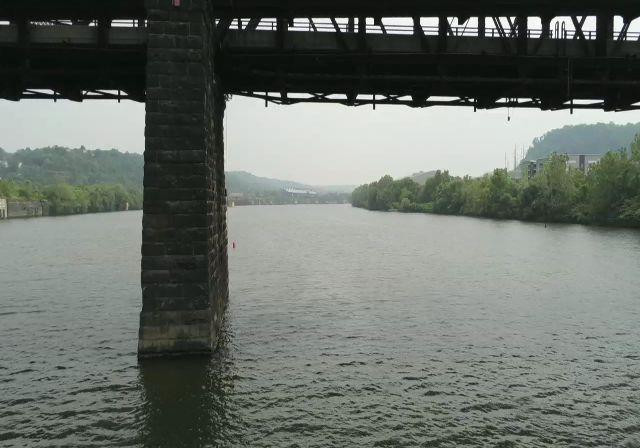
\includegraphics[width=0.95\linewidth]{chapter4/FIGS/fig-bridge-raw.jpg}\\
{\small (a) Raw Input}\\
\end{minipage}
\begin{minipage}[b]{0.495\linewidth}
\centering
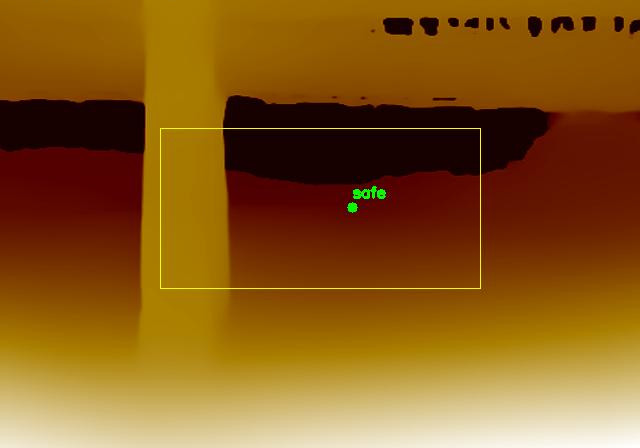
\includegraphics[width=0.95\linewidth]{chapter4/FIGS/fig-bridge-midas.jpg}\\
{\small (b) Output of MiDaS}\\
\end{minipage}
\caption{Bridge Obstacle Avoidance}
\label{fig:midas-sample}
\end{figure}

Task-5 compares my platform's monocular obstacle avoidance, using my
visual pipeline at 0.7~fps, with the stereoscopic obstacle avoidance
of the Anafi Ai using on-board computing at 30~fps.  I place the 2~m
tall by 0.5~m wide foam pillar used in Task-2~(\S\ref{sec:task2})
directly in the drone's path. The drone is instructed to fly at 1
m/s at a fixed altitude of 1~m directly towards the obstacle.  I
capture a trace of the drone's flight path across 3 different runs.

\begin{figure}
\begin{minipage}[b]{0.495\linewidth}
\centering
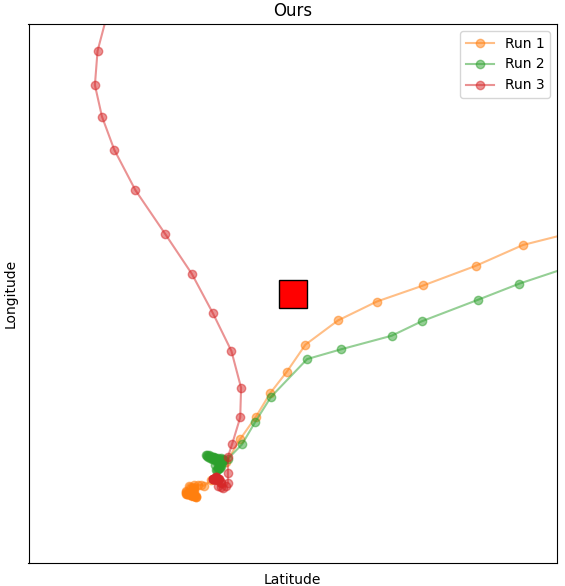
\includegraphics[width=0.95\linewidth]{chapter4/FIGS/fig-obstacle-path-ours.png}
{(a) My Platform}
\end{minipage}
\begin{minipage}[b]{0.495\linewidth}
\centering
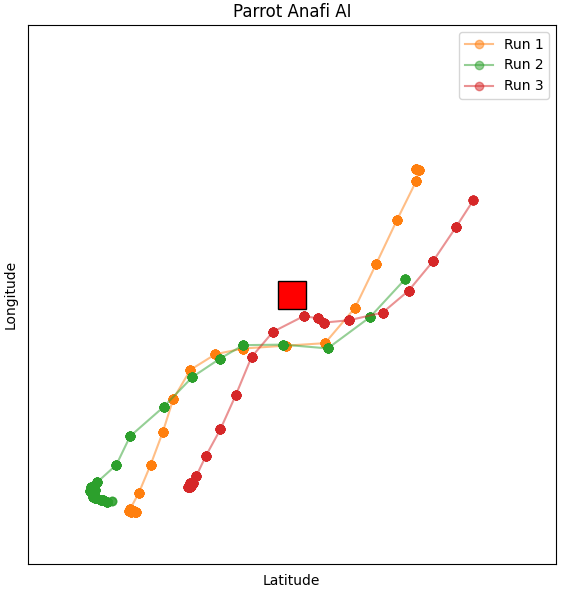
\includegraphics[width=0.95\linewidth]{chapter4/FIGS/fig-obstacle-path-anafiai.png}
{(b) Anafi Ai}
\end{minipage}
\caption{Task-5 Results}
\label{fig:obstacle-path}
\end{figure}

\subsubsection{Algorithm}
\label{sec:midas-algorithm}
Some drones utilize stereo cameras or LIDAR to detect and avoid
obstacles. These give accurate depth data (i.e., distance to objects),
allowing the drone to map out its environment and to calculate optimal
collision-free trajectories.  Since my drone is only equipped with a
monocular camera, it cannot infer depth via simple geometric methods.
I therefore use a DNN-based algorithm called MiDaS ~\cite{Ranftl2022}
to provide relative depth estimates.  Using MiDaS on each frame
received by the cloudlet, we construct the inverse relative depth map.
Based on the rate of change of relative depth across frames, we
identify obstacles in the flight path and actuate away from them.
Figure~\ref{fig:midas-sample}(a) shows an input frame from one of my
flights, as the drone approaches the obstacle course.
Figure~\ref{fig:midas-sample}(b) shows the depth-encoded output of my
algorithm on this frame.  The drone actuates towards the green dot
using a tuned PID-loop~\cite{Ang2005} to avoid the closest flags.
Once past these flags, it re-computes a new safe objective towards
which it can fly to avoid the second tier of flags.  It repeats these
steps until it is past all obstacles. This simple approach to obstacle
avoidance serves as a good experimental baseline.

\subsubsection{Results}
\label{sec:task5-results}

Figure~\ref{fig:obstacle-path}(a) plots the flight path of each run
for my platform, along with the position of the pillar.
Figure~\ref{fig:obstacle-path}(b) plots the flight paths of the Anafi
Ai on the same task.  Both platforms successfully avoid the obstacle
in all cases, but do so using very different tactics. The
low frame rate and high end-to-end latency of my pipeline forces my
platform to be very conservative, and to give the obstacle a wide
berth.  Well past the obstacle, the drone has not yet returned to its
original flight path.  In contrast, the stereoscopic cameras, high
frame rate and low end-to-end processing latency of the Anafi Ai
together enable it to be much less conservative in obstacle avoidance.
The flight paths cluster more tightly around the obstacle, and the drone
soon returns to its original flight path.

\subsection{Summary of Results}
\label{sec:take-away}

My evaluation began with a single top-level question.  Could
autonomous active vision be successfully implemented on a drone with
severe constraints on both local compute and offloading?  The maximum
offloading throughput of 0.7~fps imposed by LTE thermal constraints on
the watch~(\S\ref{sec:stream-in-practice}) is a severe bottleneck.  The
heavy-tailed distribution of end-to-end processing pipeline latency,
with a mean of over 1~s~(\S\ref{sec:event-to-detection-latency}), is another
bottleneck.  Combined with limitations of onboard processing on the
watch and the quality of the drone's optical system, these constraints
pose a formidable barrier.

In spite of this barrier, the results presented~(\S\ref{sec:task1} to
\S\ref{sec:task5}) show that active vision capabilities such as
tracking a moving object and confirming object detection by dropping
to lower altitude are feasible at credible target speeds.  Even with
the current implementation, one can perform useful tasks involving
active vision.  The range of feasible tasks can be broadened via
hardware advancements in the drone and the watch, combined with more
sophisticated algorithms that can then be supported.  Progress on this
front would also enable the superior resources of the cloudlet to be better
utilized.  Right now, the benefit of the cloudlet is being muted by the low
sustainable offloading rate. Even so, thanks to the modular design of SteelEagle, it is still possible to port new AI algorithms with minimum effort into the pipeline which could perform better on this limited stream.

\subsection{Benefit of Increased Frame Rate}
\label{sec:discussion-results}

The results for Task-3~(\S\ref{sec:task3}) make it clear that the
drone's frame rate of 0.7~fps is a major limiting factor for tracking.
When tracking high speed objects that perform erratic maneuvers, the
drone often only has one or two detections to actuate upon. It often
does not get feedback on actuation errors until the target has exited
the frame entirely. Once that happens, tracking fails and the target
is lost.

To quantify the benefits of a higher frame rate, I repeated the most
difficult combination of speed and pattern in my Task-3 experiments:
3.5~m/s for a square pattern. Instead of using the watch, I used a
ground-based laptop to play exactly the same role.  The laptop
connects to the drone over WiFi, and connects to the cloudlet via a
commercial cellular LTE network.  In every respect other than the fact
that the laptop is not flying with the drone, the processing
pipeline is unchanged from  Figure~\ref{fig:sys-arch}.
The tracking algorithm is also unchanged from that described for
Task-3~(\S~\ref{sec:task3}). Although the laptop experiences the same
WiFi, RTSP video stream, and LTE conditions as the watch did, it does
not suffer from the same processing or LTE thermal limitations.  This
enables offloading of video processing to the cloudlet a much higher frame
rate. I chose a figure of 3~fps since I believe that this is
realistically achievable with slightly better watch hardware. Even the
Samsung Galaxy 4 watch can sustain 3~fps for over two minutes if it is
pre-cooled with an ice pack.  This is the full length of one run of
Task-3~(\S~\ref{sec:task3}).

\begin{table}
        \centering\small
        \begin{tabular}{|c|c|c|c|c|c|c|}
                \hline
                Frame & Run & Total & \multicolumn{2}{c|}{Success} & Slow & Fail\\
                Rate  &  & Frames  & \multicolumn{2}{c|}{{\footnotesize (Target Present)}}& Act-  &  \\
                \cline{5-5}
                (fps) &  &         &         & $\rm \frac{Present}{Total}$  & uation  & \\
                \hline
                & 1 & 361 & 283 &        & 1 &  77 \\
                3& 2 & 360 & 342 & 83.7\% \scriptsize{(9.8\%)} & 1 & 17 \\
                & 3 & 361 & 280 &        & 0 &  82 \\
                \hline
                    & 1 & 87 & 46 & & 2 & 39 \\
                0.7 & 2 & 84 & 60 & 62.7\% \scriptsize{(9.3\%)} & 1 & 23  \\
                & 3 & 83 & 53 & & 4 & 26 \\
                \hline
        \end{tabular}
        \begin{captext}
                \centering \\[0.1cm] Speed was 3.5~m/s.  Figures in parentheses are standard deviations.
        \end{captext}
        \caption{Increased Frame Rate {\footnotesize (Altitude = 5~m, Pattern = Square)}}
        \label{tab:taskfps-results}
\end{table}

\begin{table}
        \centering\small
        \begin{tabular}{|c|c|c|}
                \hline
                Platform & Weight (g) & Throughput (fps)\\
                \hline
                Galaxy Watch 4 & 26 & 1 \\
                Future Offload Device & $<$50 & 3\\
                Pixel 4a & 143 & 5 \\
                Dell Latitude 5420 Laptop & 2500+ & 6 \\
                \hline
        \end{tabular}\\
        \caption{Throughput and Weight by Platform}
        \label{tab:throughput}
\end{table}

\begin{table}
        \centering
        \begin{tabular}{|c|c|c|c|}
                \hline
                & Inference & Effective Throughput \\
                & (ms) & (fps) \\
                \hline
                Object & 56.3 & 17.8  \\
                Detection & (5.9) &  \\
                \hline
                Obstacle & 124.3 & 8.1 \\
                Avoidance & (4.9) &  \\
                \hline
        \end{tabular}
        \begin{captext}
                \centering \\[0.1cm] Standard deviation in parentheses. \\
        \end{captext}
        \caption{Cloudlet Performance}
        \label{tab:cloudlet-perf}
\end{table}

Table~\ref{tab:taskfps-results} presents my results for an altitude of
5~m.  For easy comparison, the 3.5~m/s results from
Table~\ref{tab:task3-results-5m-square} are reproduced below the new
results.  Increasing the frame rate from 0.7~fps to 3~fps greatly
improves tracking --- almost a 20\% increase in the ``Success''
column.  Even the worst run at 3~fps achieves 77.5\% success which is
6.1\% better than the best run at 0.7~fps at 71.4\%
success.  This improvement is obtained without modifying my tracking
algorithm. 

Since frame rate is such an important factor in successful tracking,
it is natural to speculate on what might be possible with future
hardware advancements.  For example, if a future offload device was no heavier
than it is today but had the processing power of today's smartphones,
how much better could it do tracking?  To gain some insight into these
speculative questions, I tested the processing pipeline of
Figure~\ref{fig:sys-arch} using different offload platforms.  Experiments were performed with an identical setup as in Section~\ref{sec:event-to-detection-latency}.

Table~\ref{tab:throughput} shows the throughput in fps and the weight
of various computing platforms today. The first two rows are the
current platform and a theoretical future offload device.  The third row is a Pixel 4a smartphone, which is able to sustain 5~fps. At 143~g, it is too heavy
for my drone to carry, but its 5x improvement in throughput is very
attractive for robust tracking. The fourth row is a Dell Latitude 5420
laptop, which is able to sustain 6 fps; clearly, its 2.5~kg weight is
far beyond the payload lift of any ultra-light drone.  Since the
laptop can decode video and transmit it over WiFi at 30~fps, the
bottleneck shifts to the LTE link and the cloudlet's DNN inference
time.  As Table~\ref{tab:cloudlet-perf} shows, the cloudlet is able
to inference at roughly 17.8~fps for object detection~(Task-1 to
Task-4) and 8.1~fps on obstacle avoidance~(Task-5). Thus, an improved offload device on the drone could take better advantage of cloudlet resources.




